\documentclass[tikz,border=8pt]{standalone}
\usepackage[T1]{fontenc}
\IfFileExists{libertine.sty}{\usepackage{libertine}}{}
\IfFileExists{inconsolata.sty}{\usepackage[scaled=0.94]{inconsolata}}{}
\usetikzlibrary{arrows.meta,calc}

\definecolor{navy}{RGB}{35,84,135}
\definecolor{navyfill}{RGB}{241,246,251}
\definecolor{amber}{RGB}{174,106,24}
\definecolor{amberfill}{RGB}{253,248,238}
\definecolor{green}{RGB}{42,116,78}
\definecolor{greenfill}{RGB}{240,248,243}
\definecolor{ink}{RGB}{55,62,69}
\definecolor{muted}{RGB}{104,112,120}

\begin{document}
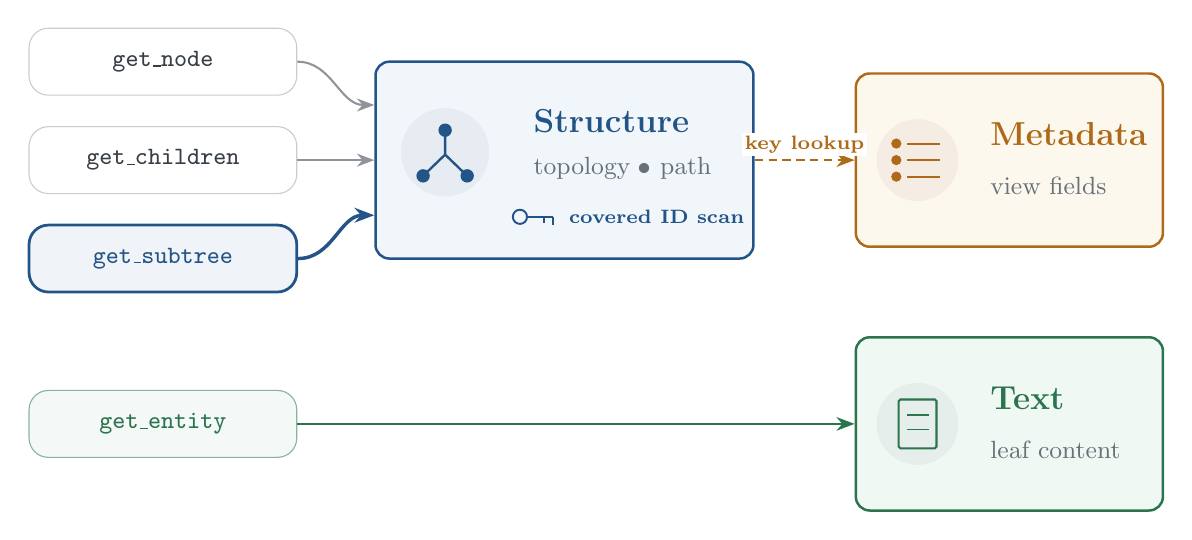
\begin{tikzpicture}[
  api/.style={
    draw=black!20, fill=white, rounded corners=7pt,
    minimum width=34mm, minimum height=8.5mm,
    font=\small\ttfamily, text=ink, align=center
  },
  hotapi/.style={api, draw=navy, fill=navy!7, line width=1pt, text=navy},
  card/.style={
    rounded corners=5pt, line width=0.9pt,
    minimum height=22mm, align=left
  },
  navflow/.style={-{Stealth[length=2.2mm]}, line width=0.75pt, draw=muted!75},
  hotflow/.style={-{Stealth[length=2.5mm]}, line width=1.25pt, draw=navy},
  metaflow/.style={-{Stealth[length=2.3mm]}, line width=0.9pt,
    draw=amber, dashed, dash pattern=on 3pt off 2pt},
  textflow/.style={-{Stealth[length=2.3mm]}, line width=0.9pt, draw=green}
]

% Storage API rail.
\node[api]    (node)     at (-5.10, 2.45) {get\_node};
\node[api]    (children) at (-5.10, 1.20) {get\_children};
\node[hotapi] (subtree)  at (-5.10,-0.05) {get\_subtree};
\node[api, draw=green!55, fill=green!5, text=green]
              (entity)   at (-5.10,-2.15) {get\_entity};

% Collection cards.
\node[
  card, draw=navy, fill=navyfill,
  minimum width=48mm, minimum height=25mm
] (structure) at (0,1.20) {};

\node[
  card, draw=amber, fill=amberfill,
  minimum width=39mm
] (metadata) at (5.65,1.20) {};

\node[
  card, draw=green, fill=greenfill,
  minimum width=39mm
] (text) at (5.65,-2.15) {};

% Structure icon: one parent and two children.
\coordinate (sicon) at ([xshift=9mm,yshift=1mm]structure.west);
\fill[navy!11] (sicon) circle (5.6mm);
\draw[navy, line width=0.85pt]
  ($(sicon)+(0,2.7mm)$) -- ($(sicon)+(0,-0.3mm)$)
  ($(sicon)+(0,-0.3mm)$) -- ($(sicon)+(-2.8mm,-3.0mm)$)
  ($(sicon)+(0,-0.3mm)$) -- ($(sicon)+(2.8mm,-3.0mm)$);
\fill[navy] ($(sicon)+(0,2.8mm)$) circle (0.85mm);
\fill[navy] ($(sicon)+(-2.8mm,-3.0mm)$) circle (0.85mm);
\fill[navy] ($(sicon)+(2.8mm,-3.0mm)$) circle (0.85mm);

\node[anchor=west, font=\large\bfseries, text=navy]
  at ([xshift=19mm,yshift=5mm]structure.west) {Structure};
\node[anchor=west, font=\small, text=muted]
  at ([xshift=19mm,yshift=-1mm]structure.west) {topology \textbullet\ path};
\coordinate (keyicon) at ([xshift=18.5mm,yshift=-7.2mm]structure.west);
\draw[navy, line width=0.7pt] (keyicon) circle (0.9mm);
\draw[navy, line width=0.7pt]
  ($(keyicon)+(0.9mm,0)$) -- ($(keyicon)+(4.2mm,0)$)
  ($(keyicon)+(3.1mm,0)$) -- ($(keyicon)+(3.1mm,-0.8mm)$)
  ($(keyicon)+(4.2mm,0)$) -- ($(keyicon)+(4.2mm,-1.0mm)$);
\node[anchor=west, font=\scriptsize\bfseries, text=navy]
  at ([xshift=23.5mm,yshift=-7.2mm]structure.west) {covered ID scan};

% Metadata icon: keyed field rows.
\coordinate (micon) at ([xshift=8mm]metadata.west);
\fill[amber!12] (micon) circle (5.2mm);
\fill[amber] ($(micon)+(-2.7mm,2.1mm)$) circle (0.65mm);
\fill[amber] ($(micon)+(-2.7mm,0)$) circle (0.65mm);
\fill[amber] ($(micon)+(-2.7mm,-2.1mm)$) circle (0.65mm);
\draw[amber, line width=0.75pt]
  ($(micon)+(-1.3mm,2.1mm)$) -- ($(micon)+(2.9mm,2.1mm)$)
  ($(micon)+(-1.3mm,0)$) -- ($(micon)+(2.9mm,0)$)
  ($(micon)+(-1.3mm,-2.1mm)$) -- ($(micon)+(2.9mm,-2.1mm)$);

\node[anchor=west, font=\large\bfseries, text=amber]
  at ([xshift=16mm,yshift=3.3mm]metadata.west) {Metadata};
\node[anchor=west, font=\small, text=muted]
  at ([xshift=16mm,yshift=-3.3mm]metadata.west) {view fields};

% Text icon: a document with two lines.
\coordinate (ticon) at ([xshift=8mm]text.west);
\fill[green!12] (ticon) circle (5.2mm);
\draw[green, line width=0.75pt, rounded corners=0.6pt]
  ($(ticon)+(-2.4mm,3.1mm)$) rectangle ($(ticon)+(2.4mm,-3.1mm)$);
\draw[green, line width=0.65pt]
  ($(ticon)+(-1.4mm,1.1mm)$) -- ($(ticon)+(1.4mm,1.1mm)$)
  ($(ticon)+(-1.4mm,-0.7mm)$) -- ($(ticon)+(1.4mm,-0.7mm)$);

\node[anchor=west, font=\large\bfseries, text=green]
  at ([xshift=16mm,yshift=3.3mm]text.west) {Text};
\node[anchor=west, font=\small, text=muted]
  at ([xshift=16mm,yshift=-3.3mm]text.west) {leaf content};

% Navigation converges on the structure collection; subtree is the hot route.
\draw[navflow] (node.east) to[out=0,in=180] ([yshift=7mm]structure.west);
\draw[navflow] (children.east) -- (structure.west);
\draw[hotflow] (subtree.east) to[out=0,in=180] ([yshift=-7mm]structure.west);

% Metadata is resolved only after IDs are selected; content bypasses navigation.
\draw[metaflow] (structure.east) -- (metadata.west)
  node[midway, above=1pt, fill=white, inner sep=1pt,
    font=\scriptsize\bfseries, text=amber] {key lookup};
\draw[textflow] (entity.east) -- (text.west);

\end{tikzpicture}
\end{document}
